%%%%%%%%%%%%%%%%%%%%%%%%%%%%%%%%%%%%%%%%%
% Lachaise Assignment
% LaTeX Template
% Version 1.0 (26/6/2018)
%
% This template originates from:
% http://www.LaTeXTemplates.com
%
% Authors:
% Marion Lachaise & François Févotte
% Vel (vel@LaTeXTemplates.com)
%
% License:
% CC BY-NC-SA 3.0 (http://creativecommons.org/licenses/by-nc-sa/3.0/)
% 
%%%%%%%%%%%%%%%%%%%%%%%%%%%%%%%%%%%%%%%%%


%----------------------------------------------------------------------------------------
%    PACKAGES AND OTHER DOCUMENT CONFIGURATIONS
%----------------------------------------------------------------------------------------

\documentclass[11pt]{article}

%%%%%%%%%%%%%%%%%%%%%%%%%%%%%%%%%%%%%%%%%
% Lachaise Assignment
% Structure Specification File
% Version 1.0 (26/6/2018)
%
% This template originates from:
% http://www.LaTeXTemplates.com
%
% Authors:
% Marion Lachaise & François Févotte
% Vel (vel@LaTeXTemplates.com)
%
% License:
% CC BY-NC-SA 3.0 (http://creativecommons.org/licenses/by-nc-sa/3.0/)
% 
%%%%%%%%%%%%%%%%%%%%%%%%%%%%%%%%%%%%%%%%%

%----------------------------------------------------------------------------------------
%    PACKAGES AND OTHER DOCUMENT CONFIGURATIONS
%----------------------------------------------------------------------------------------

\usepackage{amsmath,amsfonts,stmaryrd,amssymb} % Math packages
\usepackage{xfrac, dsfont}

\usepackage{enumerate} % Custom item numbers for enumerations

\usepackage[ruled]{algorithm2e} % Algorithms

\usepackage[framemethod=tikz]{mdframed} % Allows defining custom boxed/framed environments

\usepackage{listings} % File listings, with syntax highlighting
\lstset{
    basicstyle=\ttfamily, % Typeset listings in monospace font
}

\usepackage[
    colorlinks=true,
    linkcolor=black
]{hyperref}
\usepackage{bookmark}   % bookmarks for PDF viewing

\numberwithin{equation}{section}

%%Figure and table packages
\usepackage{booktabs,caption}
\usepackage[flushleft]{threeparttable}
\usepackage{graphicx}
\usepackage{float}
\usepackage{tabularx}
\usepackage{multirow}

\usepackage{fancyhdr}	% Header and footer control

\usepackage{minted}	% Code formatting and syntax highlighting
%\surroundwithmdframed{minted}
\definecolor{DarkGray}{rgb}{0.9, 0.9, 0.9}
\setminted{linenos=true,
    autogobble=true,
    breaklines=true, breakautoindent=true,
    bgcolor=DarkGray,
    python3=true,
    frame=lines
}
\setmintedinline{bgcolor=DarkGray}

\usepackage{chngcntr}
\counterwithin{figure}{section}

% Referencing manager
%%\usepackage[
%%	backend=biber,
%%	style=ieee
%%]{biblatex}

%----------------------------------------------------------------------------------------
%    DOCUMENT MARGINS
%----------------------------------------------------------------------------------------

\usepackage{geometry} % Required for adjusting page dimensions and margins

\geometry{
    paper=a4paper, % Paper size, change to letterpaper for US letter size
    top=2.5cm, % Top margin
    bottom=2.5cm, % Bottom margin
    left=2.5cm, % Left margin
    right=2.5cm, % Right margin
    headheight=14pt, % Header height
    footskip=1.5cm, % Space from the bottom margin to the baseline of the footer
    headsep=1.2cm, % Space from the top margin to the baseline of the header
    %showframe, % Uncomment to show how the type block is set on the page
}

%----------------------------------------------------------------------------------------
%    FONTS
%----------------------------------------------------------------------------------------

\usepackage[utf8]{inputenc} % Required for inputting international characters
\usepackage[T1]{fontenc} % Output font encoding for international characters
\linespread{1.3}        % 1.5 line spacing
\usepackage{XCharter} % Use the XCharter fonts
\usepackage[none]{hyphenat} % prevent words being split across multiple lines
\usepackage{url}

% strikethrough within math mode
\newcommand\hcancel[2][black]{\setbox0=\hbox{$#2$}%
\rlap{\raisebox{.45\ht0}{\textcolor{#1}{\rule{\wd0}{1pt}}}}#2}

%----------------------------------------------------------------------------------------
%    COMMAND LINE ENVIRONMENT
%----------------------------------------------------------------------------------------

% Usage:
% \begin{commandline}
%    \begin{verbatim}
%        $ ls
%        
%        Applications    Desktop    ...
%    \end{verbatim}
% \end{commandline}

\mdfdefinestyle{commandline}{
    leftmargin=10pt,
    rightmargin=10pt,
    innerleftmargin=15pt,
    middlelinecolor=black!50!white,
    middlelinewidth=2pt,
    frametitlerule=false,
    backgroundcolor=black!5!white,
    frametitle={Command Line},
    frametitlefont={\normalfont\sffamily\color{white}\hspace{-1em}},
    frametitlebackgroundcolor=black!50!white,
    nobreak,
}

% Define a custom environment for command-line snapshots
\newenvironment{commandline}{
    \medskip
    \begin{mdframed}[style=commandline]
}{
    \end{mdframed}
    \medskip
}

%----------------------------------------------------------------------------------------
%    FILE CONTENTS ENVIRONMENT
%----------------------------------------------------------------------------------------

% Usage:
% \begin{file}[optional filename, defaults to "File"]
%    File contents, for example, with a listings environment
% \end{file}

\mdfdefinestyle{file}{
    innertopmargin=1.6\baselineskip,
    innerbottommargin=0.8\baselineskip,
    topline=false, bottomline=false,
    leftline=false, rightline=false,
    leftmargin=2cm,
    rightmargin=2cm,
    singleextra={%
        \draw[fill=black!10!white](P)++(0,-1.2em)rectangle(P-|O);
        \node[anchor=north west]
        at(P-|O){\ttfamily\mdfilename};
        %
        \def\l{3em}
        \draw(O-|P)++(-\l,0)--++(\l,\l)--(P)--(P-|O)--(O)--cycle;
        \draw(O-|P)++(-\l,0)--++(0,\l)--++(\l,0);
    },
    nobreak,
}

% Define a custom environment for file contents
\newenvironment{file}[1][File]{ % Set the default filename to "File"
    \medskip
    \newcommand{\mdfilename}{#1}
    \begin{mdframed}[style=file]
}{
    \end{mdframed}
    \medskip
}

%----------------------------------------------------------------------------------------
%    NUMBERED QUESTIONS ENVIRONMENT
%----------------------------------------------------------------------------------------

% Usage:
% \begin{question}[optional title]
%    Question contents
% \end{question}

\mdfdefinestyle{question}{
    innertopmargin=1.2\baselineskip,
    innerbottommargin=0.8\baselineskip,
    roundcorner=5pt,
    nobreak,
    singleextra={%
        \draw(P-|O)node[xshift=1em,anchor=west,fill=white,draw,rounded corners=5pt]{%
        Question \theQuestion\questionTitle};
    },
}

\newcounter{Question} % Stores the current question number that gets iterated with each new question

% Define a custom environment for numbered questions
\newenvironment{question}[1][\unskip]{
    \bigskip
    \stepcounter{Question}
    \newcommand{\questionTitle}{~#1}
    \begin{mdframed}[style=question]
}{
    \end{mdframed}
    \medskip
}

%----------------------------------------------------------------------------------------
%    WARNING TEXT ENVIRONMENT
%----------------------------------------------------------------------------------------

% Usage:
% \begin{warn}[optional title, defaults to "Warning:"]
%    Contents
% \end{warn}

\mdfdefinestyle{warning}{
    topline=false, bottomline=false,
    leftline=false, rightline=false,
    nobreak,
    singleextra={%
        \draw(P-|O)++(-0.5em,0)node(tmp1){};
        \draw(P-|O)++(0.5em,0)node(tmp2){};
        \fill[black,rotate around={45:(P-|O)}](tmp1)rectangle(tmp2);
        \node at(P-|O){\color{white}\scriptsize\bf !};
        \draw[very thick](P-|O)++(0,-1em)--(O);%--(O-|P);
    }
}

% Define a custom environment for warning text
\newenvironment{warn}[1][Warning:]{ % Set the default warning to "Warning:"
    \medskip
    \begin{mdframed}[style=warning]
        \noindent{\textbf{#1}}
}{
    \end{mdframed}
}

%----------------------------------------------------------------------------------------
%    INFORMATION ENVIRONMENT
%----------------------------------------------------------------------------------------

% Usage:
% \begin{info}[optional title, defaults to "Info:"]
%     contents
% \end{info}

\mdfdefinestyle{info}{%
    topline=false, bottomline=false,
    leftline=false, rightline=false,
    nobreak,
    singleextra={%
        \fill[black](P-|O)circle[radius=0.4em];
        \node at(P-|O){\color{white}\scriptsize\bf i};
        \draw[very thick](P-|O)++(0,-0.8em)--(O);%--(O-|P);
    }
}

% Define a custom environment for information
\newenvironment{info}[1][Info:]{ % Set the default title to "Info:"
    \medskip
    \begin{mdframed}[style=info]
        \noindent{\textbf{#1}}
}{
    \end{mdframed}
}

\usepackage{XCharter} % Include the file specifying the document structure and custom commands

\usepackage{draftwatermark}
\SetWatermarkText{\textsf{\textbf{CONFIDENTAL}}}
\SetWatermarkScale{2.5}
\SetWatermarkColor[gray]{0.8}
\SetWatermarkAngle{50}

\pagestyle{fancy}
\fancyhf{}
\renewcommand{\headrulewidth}{2pt}
\renewcommand{\footrulewidth}{1pt}
\lhead{\textit{Certificate Maker Kickstart Manual}}
\rhead{\leftmark}
\cfoot{Page \thepage}

%----------------------------------------------------------------------------------------
%    ASSIGNMENT INFORMATION
%----------------------------------------------------------------------------------------

\title{Certificate Maker Kickstart Manual} % Title of the assignment

\author{Harrison Outram\\ Membership Officer}

\date{Curtin IET On Campus --- \today} % University, school and/or department name(s) and a date

%----------------------------------------------------------------------------------------

\begin{document}

%----------------------------------------------------------------------------------------
%    TITLE PAGE
%----------------------------------------------------------------------------------------

\begin{titlepage} % Suppresses displaying the page number on the title page and the subsequent page counts as page 1
    \newcommand{\HRule}{\rule{\linewidth}{0.5mm}} % Defines a new command for horizontal lines, change thickness here
    
    \center % Centre everything on the page
    
    %------------------------------------------------
    %    Headings
    %------------------------------------------------
    
    \textsc{\LARGE Curtin IET On Campus}\\[1.5cm] % Main heading such as the name of your university/college
    
    \textsc{\LARGE Institute of Engineering and Technology}\\[0.5cm] % Major heading such as course name
    
    %------------------------------------------------
    %    Title
    %------------------------------------------------
    
    \HRule\\[0.4cm]

    \vspace{0.4cm}
    
    {\Huge\bfseries Certificate Maker Kickstart Manual}\\[0.4cm] % Title of your document
    
    \HRule\\[1.5cm]
    
    %------------------------------------------------
    %    Author(s)
    %------------------------------------------------
    
    \begin{center}
        \large
        Harrison G. Outram \\
        Membership Officer
    \end{center}
    
    %------------------------------------------------
    %    Date
    %------------------------------------------------
    
    \vfill\vfill\vfill % Position the date 3/4 down the remaining page
    
    {\Large\today} % Date, change the \today to a set date if you want to be precise
    
    %------------------------------------------------
    %    Logo
    %------------------------------------------------
    
    \vfill
    
\includegraphics[width=0.8\textwidth]{../../assets/IET_Logo_Blue_RGB.pdf}\\
     
    %----------------------------------------------------------------------------------------
    
    \vfill % Push the date up 1/4 of the remaining page
    
\end{titlepage}

\pagenumbering{roman}

\tableofcontents

\bigskip

\listoffigures

\newpage

%----------------------------------------------------------------------------------------
%    INTRODUCTION
%----------------------------------------------------------------------------------------

\pagenumbering{arabic}
\setcounter{page}{1}

\section{Introduction}

\subsection{Context}

Curtin IET On Campus (or ``CIET'' for short) provides multiple industry talks and workshops to STEM students (particularly engineering and computer related science). As part of CIET's commitment to quality, attendees shall recieve a certificate of attendance stating the name of the event, the club name, the president's full name with a signature, the the attendee's full name, and the number of approved CPD hours. This certificate of attendance must be done in a PDF document with vector graphics where possible, then emailed to attendees as soon as possible. This is particularly important for undergraduate engineering students, as one graduation requirement is to obtain a minimum of 16 weighted hours (or five and a third actual) in the PRES category (technical presentations and workshops by a professional body). By creating and sending out these certificates, CIET is holding itself to a high standard of attendee satisfaction and professional development.

\subsection{Problem}

Despite the necessity of creating and sending certificates, the process for doing so is extremely time consuming and error prone. As shown in Figure \ref{fig:old-solution}, this process is comprised of four stages: (1) the attendee record must be collected from the events team and checked for errors, e.g. multiple registrations from one person or missing but required information. (2) one certificate is made for each attendee via the template on CIET's Canva account. Each certificate is then checked one by one for errors, being recreated if erroneous. (3) the certificates are uploaded to CIET's MailChimp account, where MailChimp auto-generates a URI for each certificate, required later on. Unfortunately, these URIs involve a randomly generated hexadecimal string, meaning each URI must be recorded manually in the attendee record, then checked for errors. Once the attendee record has been updated with certificate URIs, it is uploaded to MailChimp. (4) The certificates are checked one last time by creating a mock campaign on MailChimp, going through each attendee, downloading the certificate, then checking the certificate for errors and fixing where erroneous. All up, this process takes at least two hours per 50 attendees for someone who has gone through it before, and \textbf{far} longer for someone who has not. Worse yet, despite every certificate being checked three times during this process, it is still possible for erroneous certificates to be sent out, which has happened on at least one occasion. Clearly, this process is extremely time consuming and error prone, leading to attendee frustration and a negative impact on CIET's reputation.

\newpage

\begin{figure}[h!]
    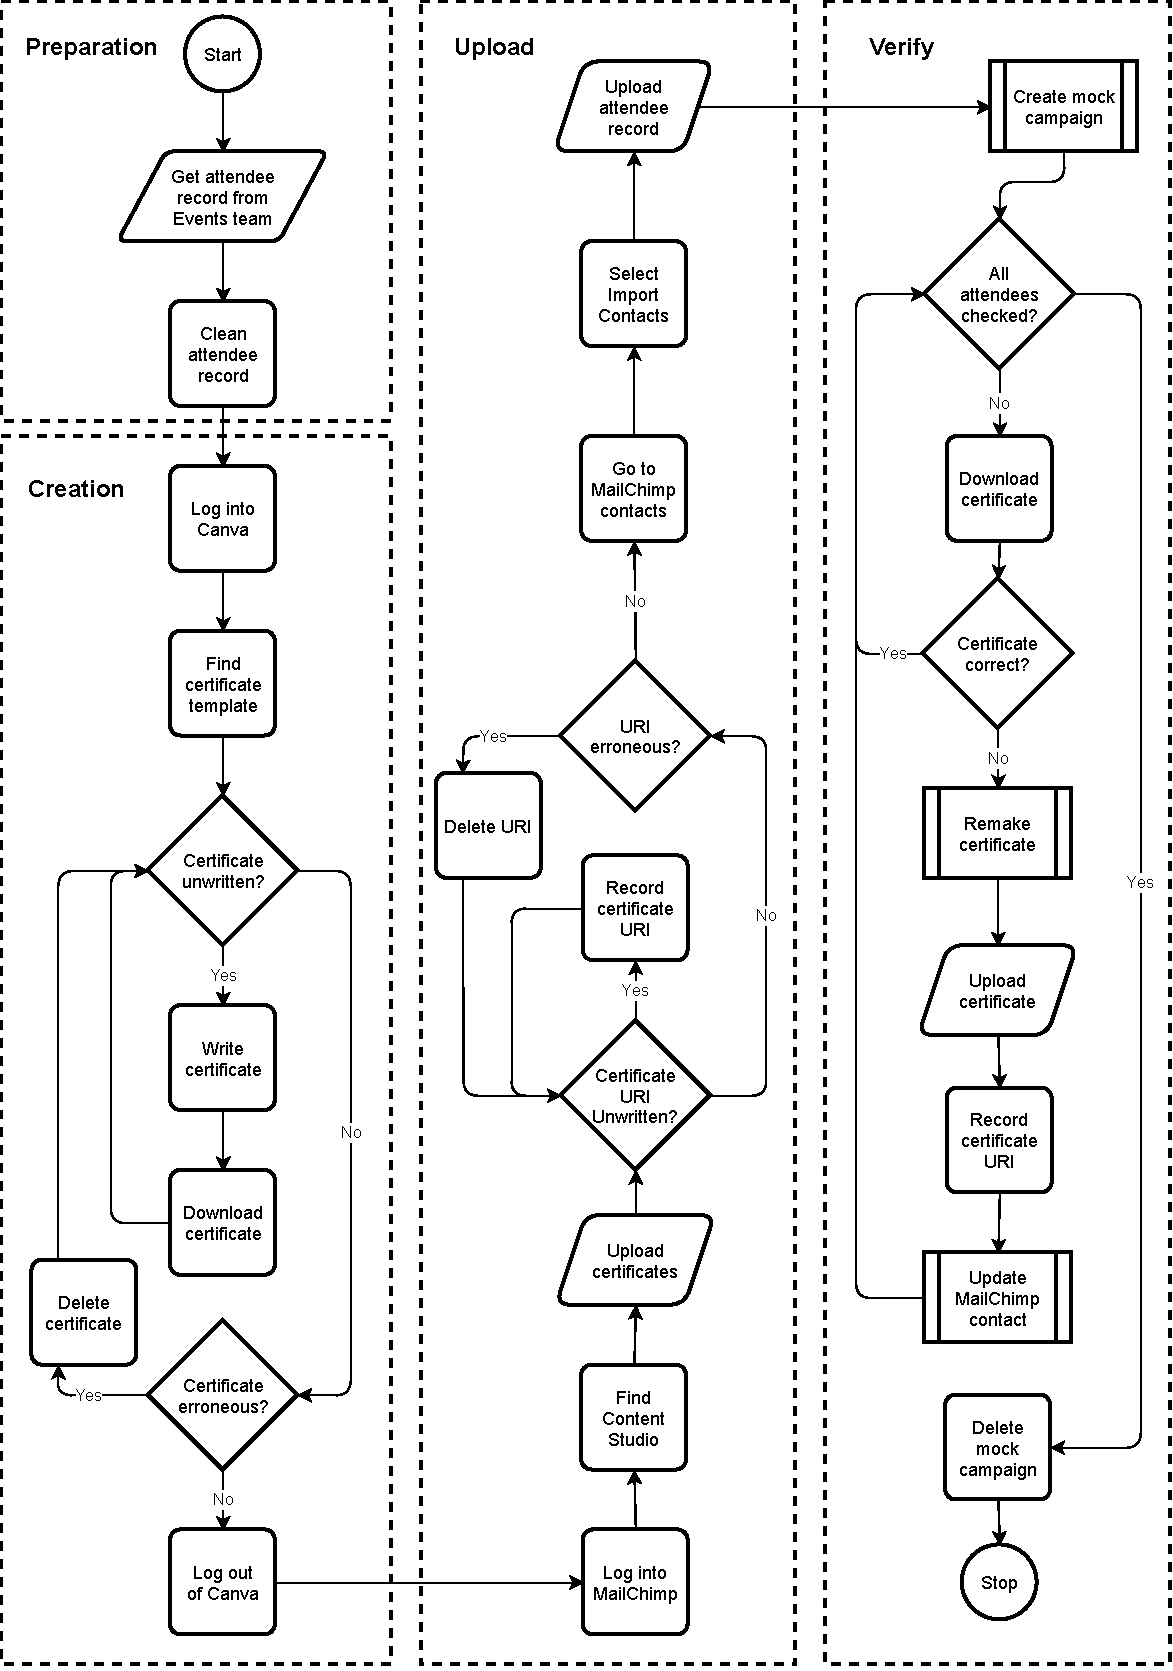
\includegraphics[width=\textwidth]{figures/old_solution.pdf}
    \caption{Old solution flowchart.}
    \label{fig:old-solution}
\end{figure}

\newpage

\section{Solution Overview}

\subsection{Rundown}

After some research, it has been discovered that stages 2, 3, and 4 of the old solution can be automated. For stage 1, instead of logging into Canva and creating each certificate manually, the template can be downloaded once and used to automatically create every certificate. The MailChimp API can be used to automatstage 3, where each certificate can be uploaded and have its URI recorded. With the URIs known, the attendee record can be updated and uploaded to MailChimp. Since the certificates were created automatically, stage 4 becomes redundant. This process is sumarised in figure \ref{fig:new-solution}. With such a script, CIET can be confident in its ability to deliver the correct certificates to its members on time and without significant human time investments.

\begin{figure}[b!]
    \centering
    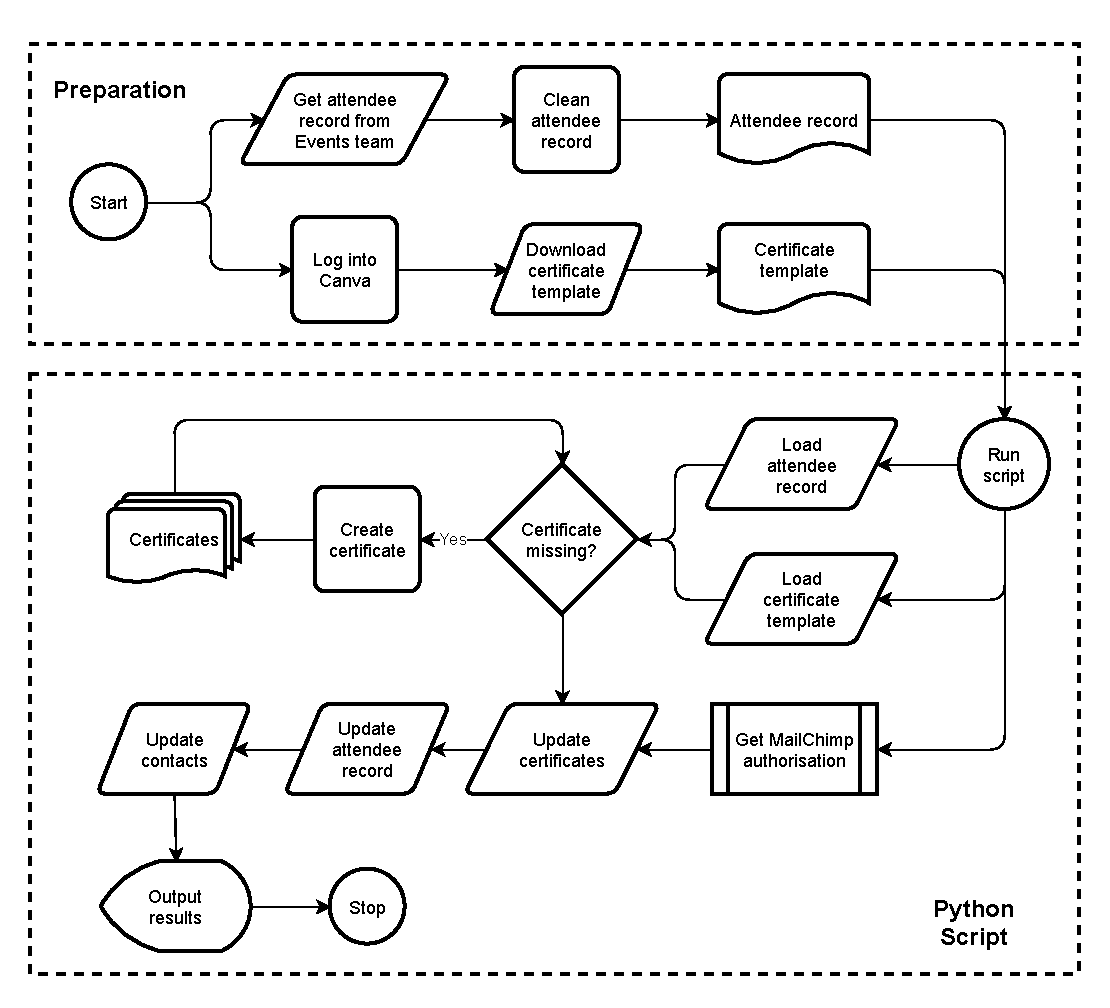
\includegraphics[width=0.8\textwidth]{figures/new_solution.pdf}
    \caption{New solution flowchart.}
    \label{fig:new-solution}
\end{figure}

Realising this goal, however, will require a well organised team and a plan. Due to the various actions this script must perform, a moderately large codebase utilising several libraries and protocols is needed, demanding a significant time investment and expertise. This complexity is compounded by delegating the workload between a team, needing appropriate version control, task management, and enforeable coding standards. Furthermore, such a project could easily suffer from scope creep, especially with the user interface. Hence, the need for subsequent sections in this document to eliminate these issues.

\subsection{Minimal Viable Product}



\subsection{Professional Product}



\subsection{Ideal Product}



\newpage

\section{Prerequisite Knowledge}

\subsection{Python Language}



\subsection{HTTP Requests and Responses}



\subsection{Application Programming Interface}



\newpage

\section{PDF Editing and Creation}



\newpage

\section{MailChimp Authorisation}

\subsection{Using API and Server Keys}




\subsection{Using OAuth 2.0}



\newpage

\section{Certificate Uploading}




\newpage

\section{Contact Updating}



\newpage

\section{User Interface}

\subsection{Command Line Interface}






\subsection{Desktop GUI}




\subsection{Web App}



\newpage

\section{Version Control}

\subsection{What is Git?}



\subsection{Using Github}



\subsection{Recording Library Requirements}



\subsection{Virtual Environments}



\newpage

\section{Coding Standards}

\subsection{Readability and Maintainability}



\subsection{Documentating using Sphinx}



\newpage

%%\printbibliography

\end{document}